



\section{Obtaining the framed Link}
Given $\mathcal{H}_{n}^\star$ into
$\mathbb{R}^3$ we obtain the $k$-component 
framed link (corresponding to the $k$ twistors) as a set of 
PL-triangulated $k$ cylinders in the 2-skeleton of 
$\mathcal{H}_{n}^\star$, named $\mathcal{C}_1,$ $\mathcal{C}_2, \ldots,\mathcal{C}_k$.
Observe that at this stage every 0-simplex of  $\bigcup_{j=1}^k \mathcal{C}_j$ 
has a 3-D coordinate attached to it. These cylinders are parametrized
as $k$ pairs of isometric rectangles (forming a strip) as in Fig. \ref{fig:strips}.
We draw $k$ straight horizontal lines at different heights of the rectangles, in the example,
lines $c_1-c_1$, $c_2-c_2$ and $c_3-c_3$. These lines are 
mapped into polygons in $\mathbb{R}^3$ which are PL-closed curves. 
The data we need is $\bigcup_{j=1}^k \mathcal{C}_j \subset \mathcal{H}_{n}^\star$
and we can discard the rest of $\mathcal{H}_{n}^\star$. The link that we seek 
is $\bigcup_{j=1}^k c_j$ with framing $\ell_j$, where $\ell_j$ is
given by the linking number of the two components of $\mathcal{C}_j$ oriented in
the same (arbitrary) direction.
We briefly review the definition of linking number 
\cite {lickorish1997introduction}.
Consider two distinct components $K_1$ and $K_2$ of an oriented link projected into
the plane so that the crossings are transversal 
(no tangency) and that there are no triple points. 
The projection is also {\em decorated}
in the sense that at each crossing the upper and 
the lower strands are given, usually,
by omitting a small segment of the lower strand.
 The \index{linking number} {\em linking number} of $\{K_1, K_2\}$
is half of the algebraic sum of the signs of the crossings 
between $K_1$ and $K_2$, oriented 
in the same direction. If $G$ is a gem, $|G|$ means
the 3-manifold induced by $G$.
The link projection given in Fig. \ref{fig:projecoes2} 
which induce $|r^{24}_5|$ has its three linking numbers $-3$.




%----------------------


\begin{proposition}
\label{prop:totalnumberofsimplices}
 The number of 1-simplices in $\bigcup_{j=1}^k c_j$ is 
at most $12n^2$, where $2n$ is the number
of vertices of the input gem.
\end{proposition}
\begin{proof} 
 A $c_j$ crosses one PL2$_m$-face, for $m\in \{0,1,2,3\}$.
 It is easy to verify that the maximum number of 2-simplices in $B_i'$ or $ P'_i$ is
 $3i-1$ and this number exceeds similar numbers for $B_i$, $ P_i$, $R^b_i$ and $R^p_i$, for 
 $i \ge  1$. The maximum $i$ is $2n-1$, so the maximum number of 2-simplices 0-, 1- and 2-colored in one PL2-face of the 
 final complex is $6n-4$. Each 1-simplex of $c_j$ crosses at most once each 2-simplex.
 Therefore, the number of 1-simpices crossing a 2-simplex 0-, 1- and 2-colored is at most $12n-8$. 
 A $c_j$ crosses at most four 2-simplices 3-colored. The result follows because $n$ is an upper 
 bound for $k$, number of components. Just note that a component in the link
 is in 1-1 correspondence with the twistors of the original gem and a twistor 
is formed by 2 vertices. This proof is partially ilustrated in Fig. \ref{fig:strips}.
 The illustration is not faithful because we can replace the strips at the right by
their bottom parts, getting simpler cylinders homotopic to the ones illustrated.
\end{proof}

Each cylinder is formed by two strips. Each strip by two adequate
pairs of two PL2-faces in the boundary of the PL3-faces in the hinge.
In the way depicted we have one PL3-face of each color $c$, $c=0,1,2,3$.
The number of  crossings of the curves $c_j$, $j=1,2,3$ coincides with the
number of $1$-simplices (or $0$-simplices) of $\bigcup_{j=1}^3 \mathcal{C}_j$.
To decrease this number we can replace the part of the strip which does not use a
PL2$_3$-face by the two complementary PL2$_3$-faces in the corresponding PL3-face.
This produces isotopic cylinders, but the number of crossings of the $c_j$'s are smaller. 
Note that each PL2$_3$-face has just five 2-simplices. In Fig. \ref{fig:strips} we 
depict the situation for the wings arising from $r_5^{24}$ before the 3 replacements.


\begin{figure}[!htb]
\begin{center}
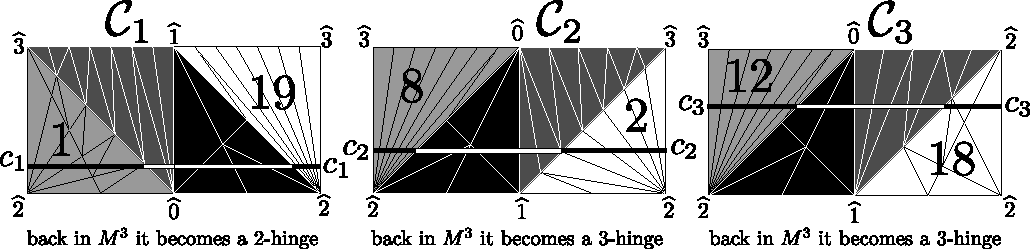
\includegraphics[width=15cm]{A.figs/strips.pdf}
\caption{From hinges to cylinders 
$\mathcal{C}_j$  to curves  $c_j$ (example inducing  $|r^{24}_5|$).
%Each cylinder is formed by two strips. Each strip by two adequate
%pairs of two PL2-faces in the boundary of the PL3-faces in the hinge.
%In the way depicted we have one PL3-face of each color $c$, $c=0,1,2,3$.
%The number of  crossings of the curves $c_j$, $j=1,2,3$ coincides with the
%number of $1$-simplices (or $0$-simplices) of $\bigcup_{j=1}^3 \mathcal{C}_j$.
%To decrease this number we can replace the right part of each strip by the
%two complementary faces at each right PL3-face. This produce isotopic cylinders,
%but the number of crossings of the $c_j$'s are smaller.
}  
\label{fig:strips}
\end{center}
\end{figure}

%----------------------
\begin{figure}[!htb]
\begin{center}
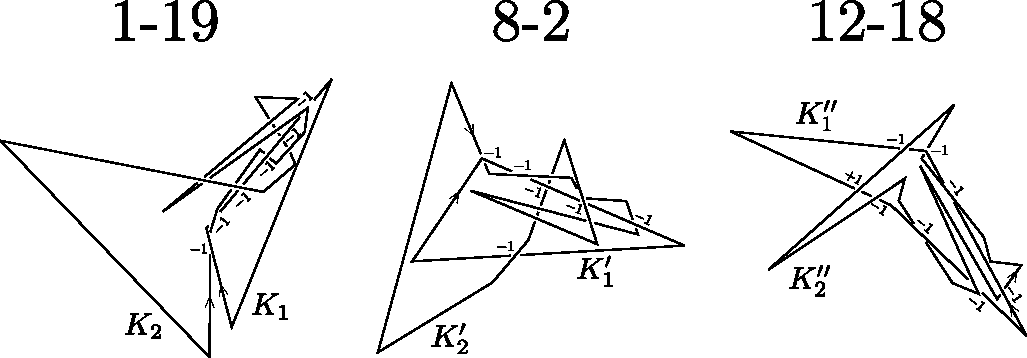
\includegraphics[scale=0.9]{A.figs/projecoes2.pdf}
\caption{Projection of the algorithm's output, yielding 
the linking numbers of the 
boundary components of the embedded cylinders of Fig. \ref{fig:strips}.}
\label{fig:projecoes2}
\end{center}
\end{figure}




